\subsection{Baza danych}
Na rysunku \ref{diagram} przedstawiony jest diagram ER schematu bazy danych.
\begin{figure}[H]
\centering
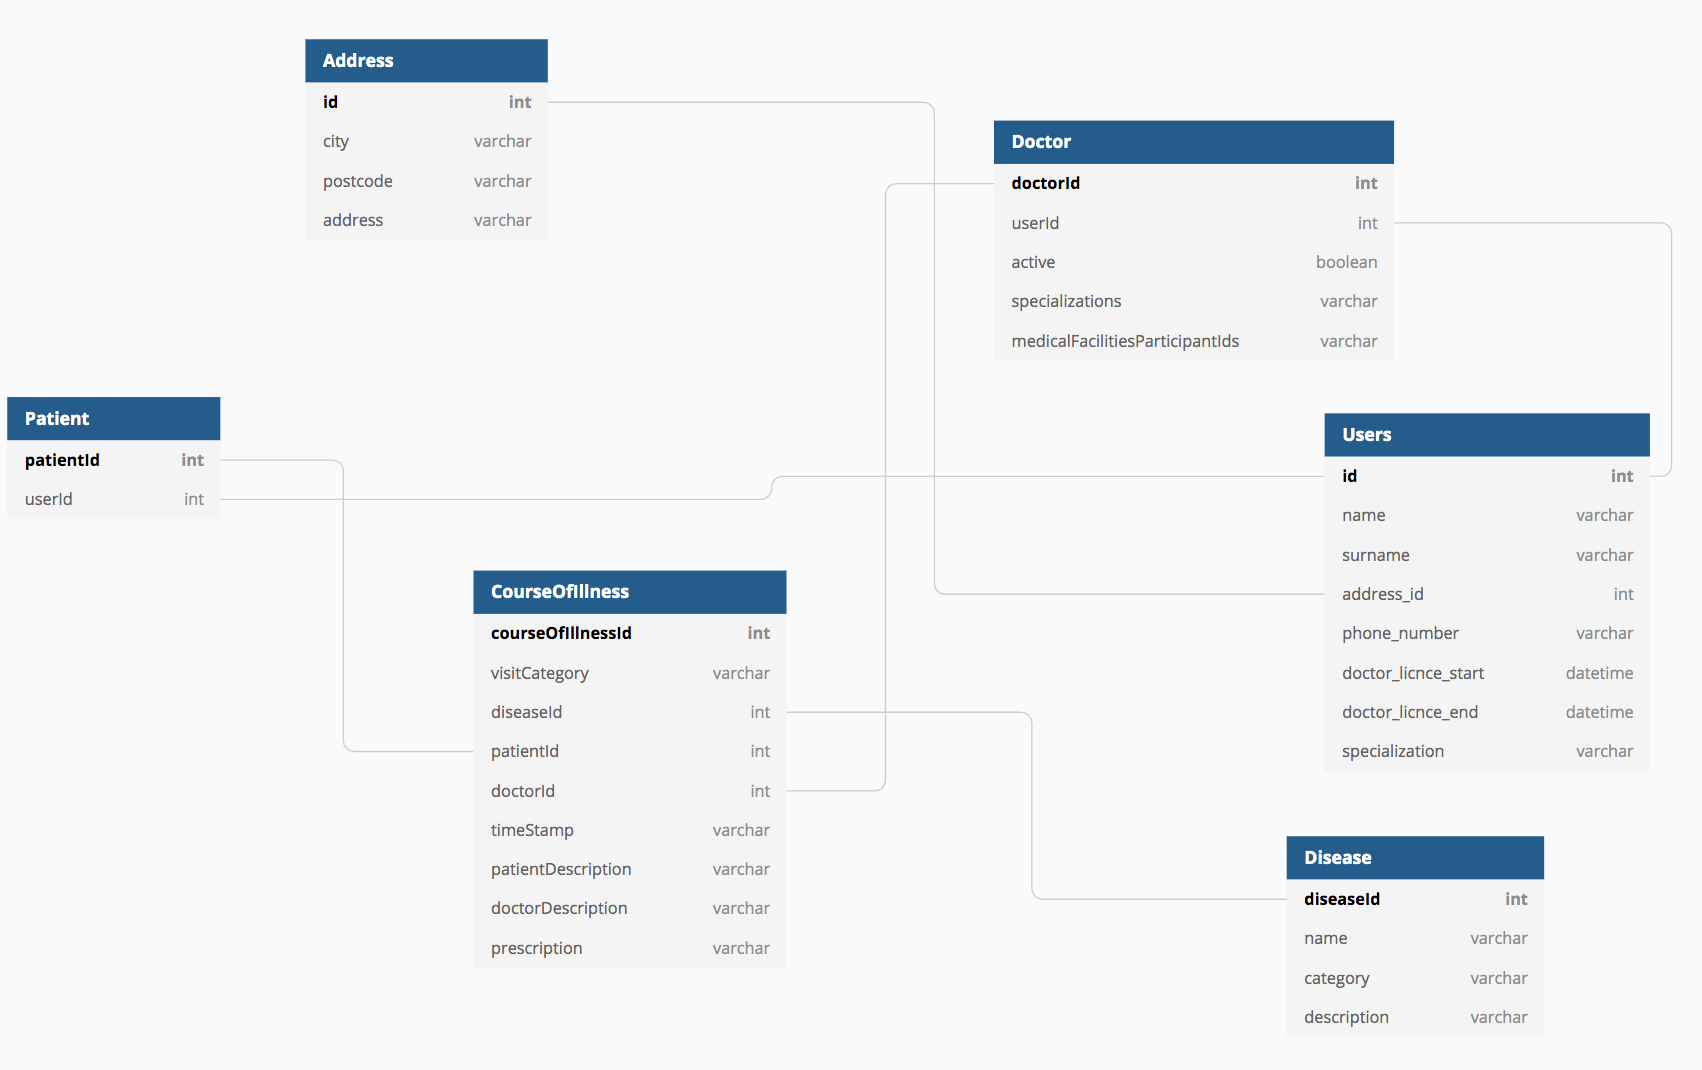
\includegraphics[width=15cm]{pictures/diagram}
\caption{Diagram ER bazy danych}
\label{diagram}
\end{figure}


Poniżej przedstawiono kod SQL wykorzystywany do inicjalizacji bazy danych:
\begin{lstlisting}[
           language=SQL,
           showspaces=false,
           basicstyle=\ttfamily,
           numbers=left,
           numberstyle=\tiny,
           commentstyle=\color{gray}
        ]
CREATE TABLE "Address" (
  "id" SERIAL PRIMARY KEY NOT NULL,
  "city" varchar,
  "postcode" varchar,
  "address" varchar
);

CREATE TABLE "Users" (
  "id" SERIAL PRIMARY KEY NOT NULL,
  "name" varchar,
  "surname" varchar,
  "address_id" int,
  "phone_number" varchar,
  "doctor_licnce_start" datetime,
  "doctor_licnce_end" datetime,
  "specialization" varchar
);

CREATE TABLE "Disease" (
  "diseaseId" SERIAL PRIMARY KEY NOT NULL,
  "name" varchar,
  "category" varchar,
  "description" varchar
);

CREATE TABLE "Doctor" (
  "doctorId" int PRIMARY KEY,
  "userId" int,
  "active" boolean,
  "specializations" varchar,
  "medicalFacilitiesParticipantIds" varchar
);

CREATE TABLE "Patient" (
  "patientId" int PRIMARY KEY,
  "userId" int
);

CREATE TABLE "CourseOfIllness" (
  "courseOfIllnessId" int PRIMARY KEY,
  "visitCategory" varchar,
  "diseaseId" int,
  "patientId" int,
  "doctorId" int,
  "timeStamp" varchar,
  "patientDescription" varchar,
  "doctorDescription" varchar,
  "prescription" varchar
);

ALTER TABLE "Users" 
ADD FOREIGN KEY ("address_id") 
REFERENCES "Address" ("id");

ALTER TABLE "Doctor" 
ADD FOREIGN KEY ("userId") 
REFERENCES "Users" ("id");

ALTER TABLE "Patient" 
ADD FOREIGN KEY ("userId") 
REFERENCES "Users" ("id");

ALTER TABLE "CourseOfIllness" 
ADD FOREIGN KEY ("diseaseId") 
REFERENCES "Disease" ("diseaseId");

ALTER TABLE "CourseOfIllness" 
ADD FOREIGN KEY ("patientId") 
REFERENCES "Patient" ("patientId");

ALTER TABLE "CourseOfIllness" 
ADD FOREIGN KEY ("doctorId") 
REFERENCES "Doctor" ("doctorId");
\end{lstlisting}

